\subsection{Experimental Setup}

In order to investigate the efficiency of CTNN cells we setup a simple (and rather classical in the RL literature \cite{cartpoleSutton}) motor control experiment: the cart-pole problem. We use the \textit{Mujoco} gym implementation of cart-pole together with our \textit{DERL} implementation of \textit{PPO} training for CTNN policies to perform our experiments. We use the adjoint method for the computation of gradients and focus our experiments on \textit{LTC cells}. The code used for the experiments is publicly available at \url{https://github.com/RenardDesNeiges/CTNN_Policies_DERL}.\\

\begin{figure}[h!]
    \centering
    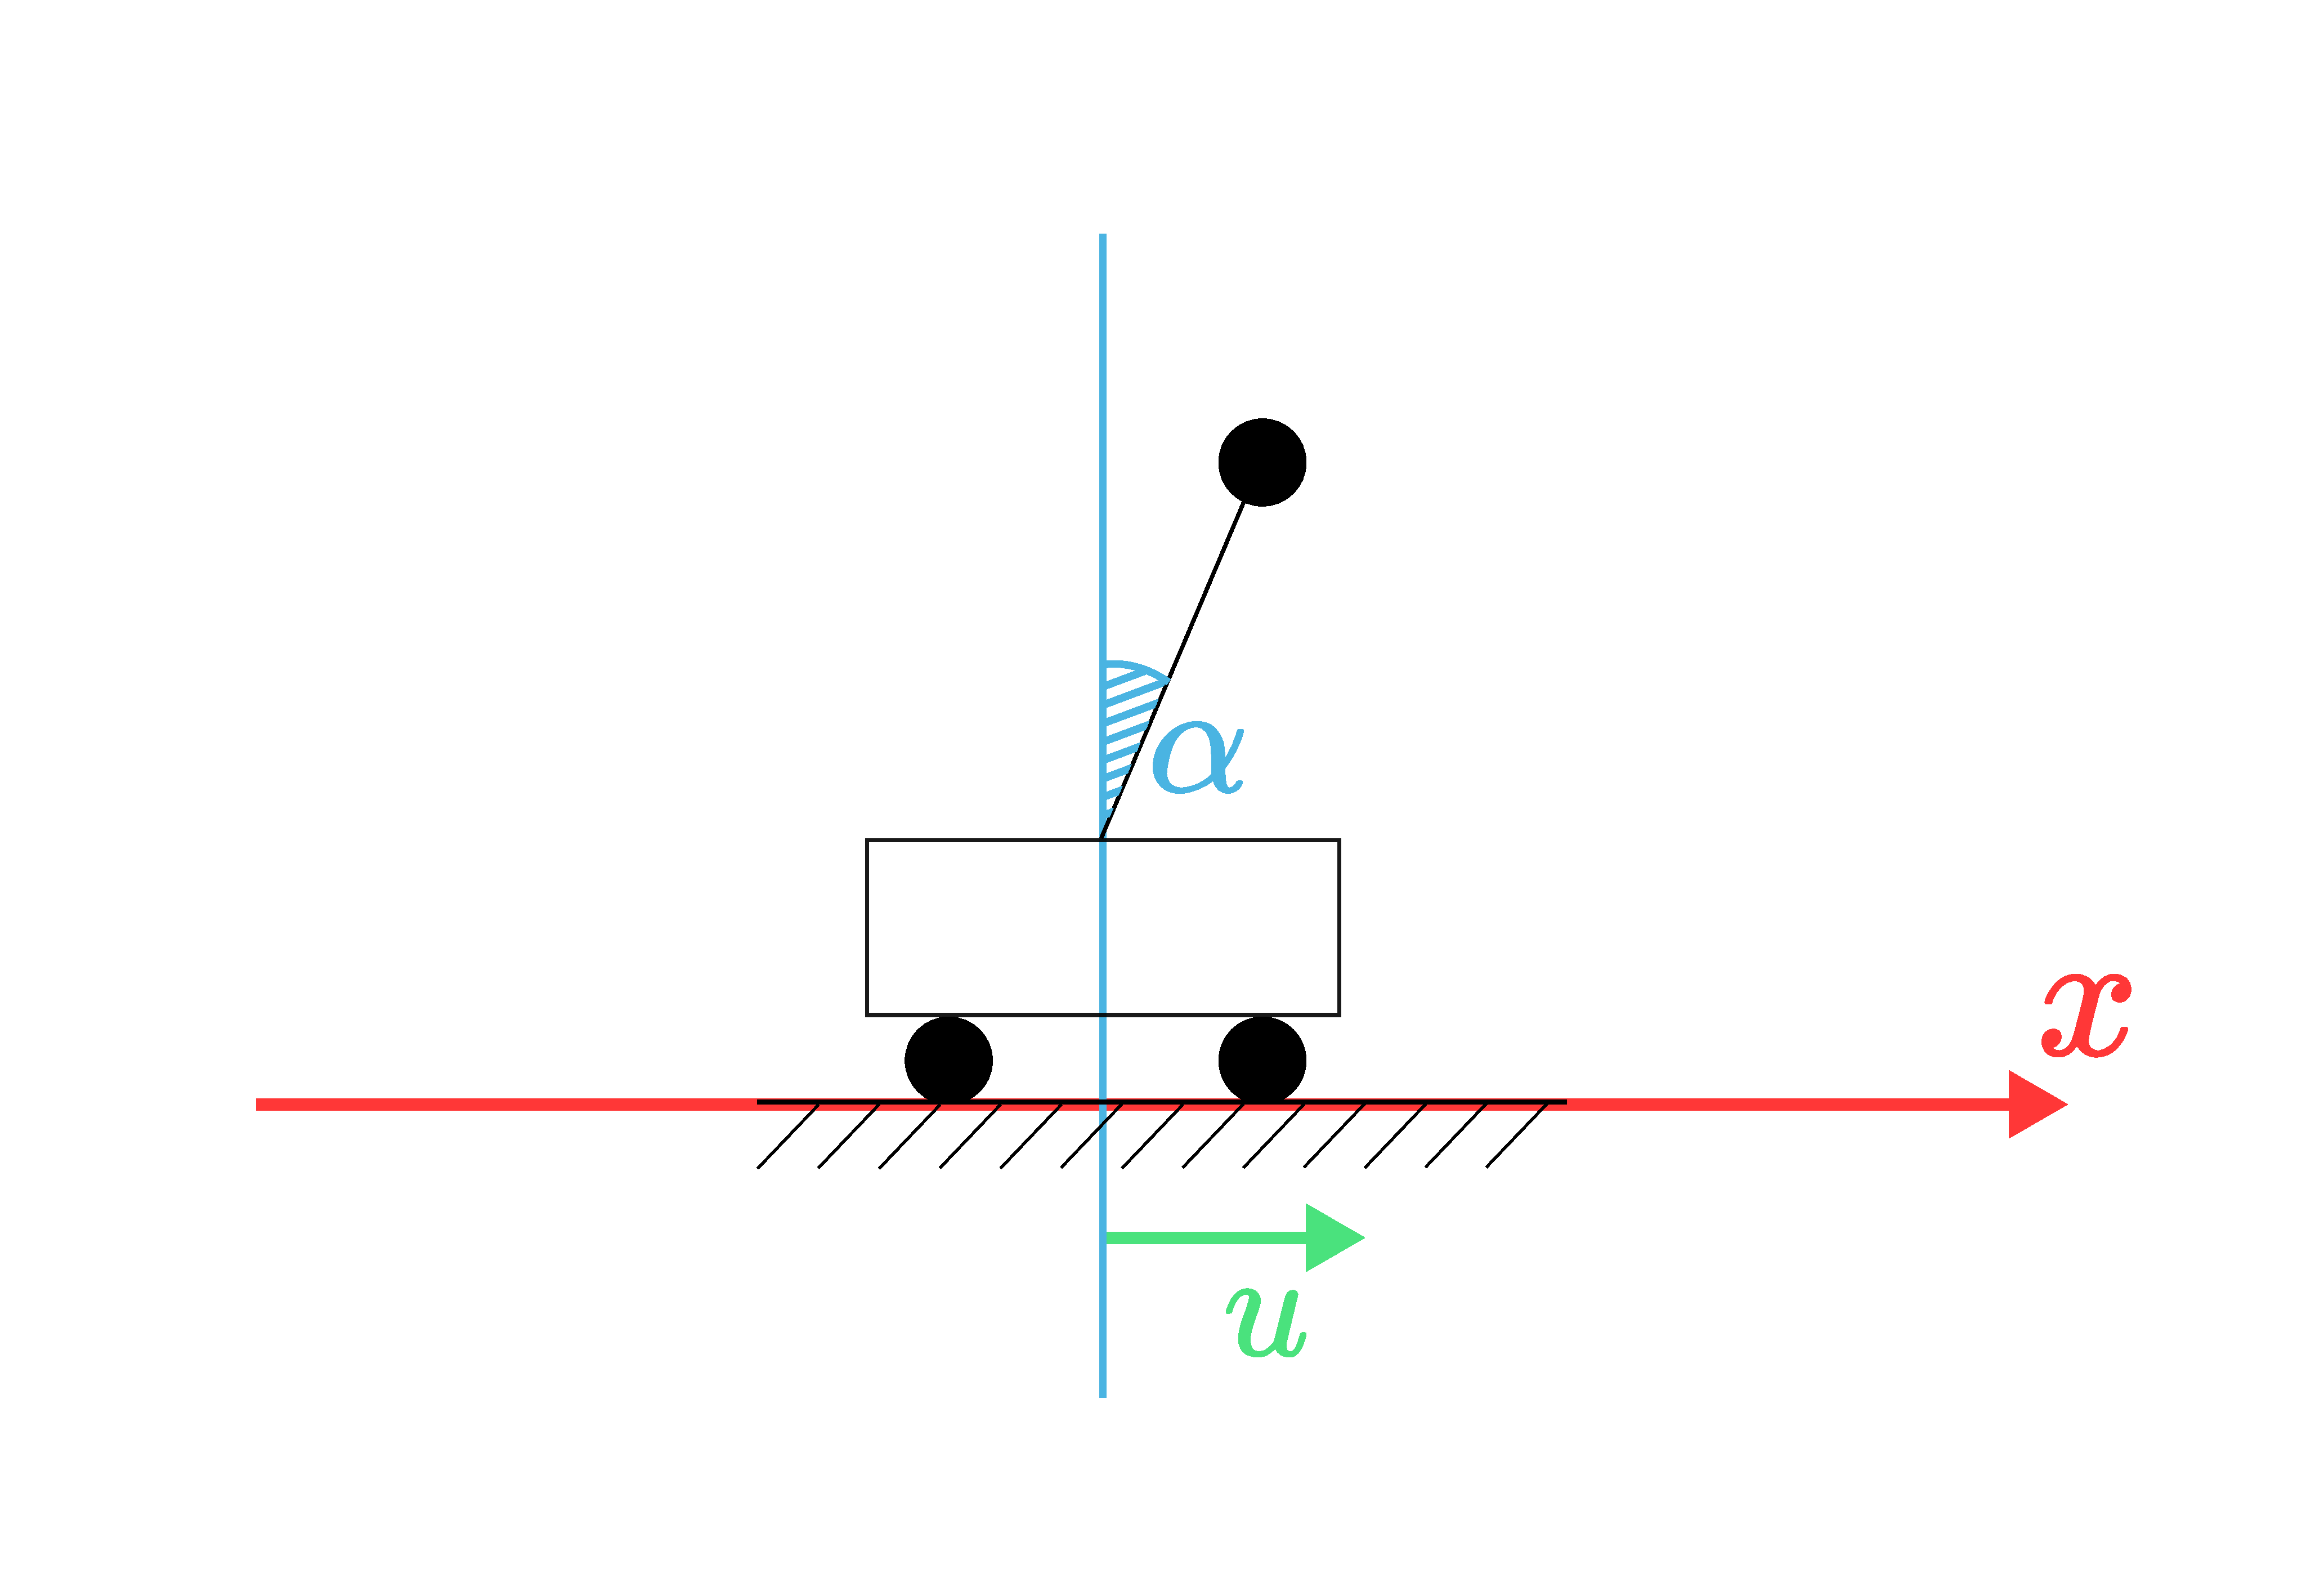
\includegraphics[width=0.4\textwidth]{figures/cartpole.pdf}
    \caption{The cart-pole system, with both coordinates $x$ and $\alpha$, as well as the control variable $u$ (a linear force on the cart) clearly labeled.}
    \label{fig:cartpole_scheme}
\end{figure}

The cart-pole problem is characterized by a 4-dimensional continuous observation space given by $o(t)=[\alpha,x,\dot{\alpha},\dot{x}]$ and a single dimensional continuous action space which we denote as $a(t) = u$ (see figure \ref{fig:cartpole_scheme}). For all of our cart-pole experiments we use the following reward: 

\begin{align*}
    r_t = 
    \begin{cases}
        -2 & \text{if} ~|\alpha|>\alpha_\text{max} ~\text{(failure)}\\
        1-q u^2 & \text{otherwise} 
    \end{cases}
\end{align*}

Where $q=0.2$ is a penalty on control (where $u$ is a force measured in newtons) and where the angle $\alpha_\text{max}=0.209$ is used to define failure (with $\alpha$ the pole-angle measured in radiant). The cart-pole implementation we use has a limited range of motion in $x$ (when the cart reaches the end of it's range of motion it cannot go further which means a well tuned policy should learn to avoid the edges). Together with the observation space, the action space and the stochastic transition probability function defined by the physics simulation this defines a POMDP. \\

\begin{figure}[h!]
    \centering
    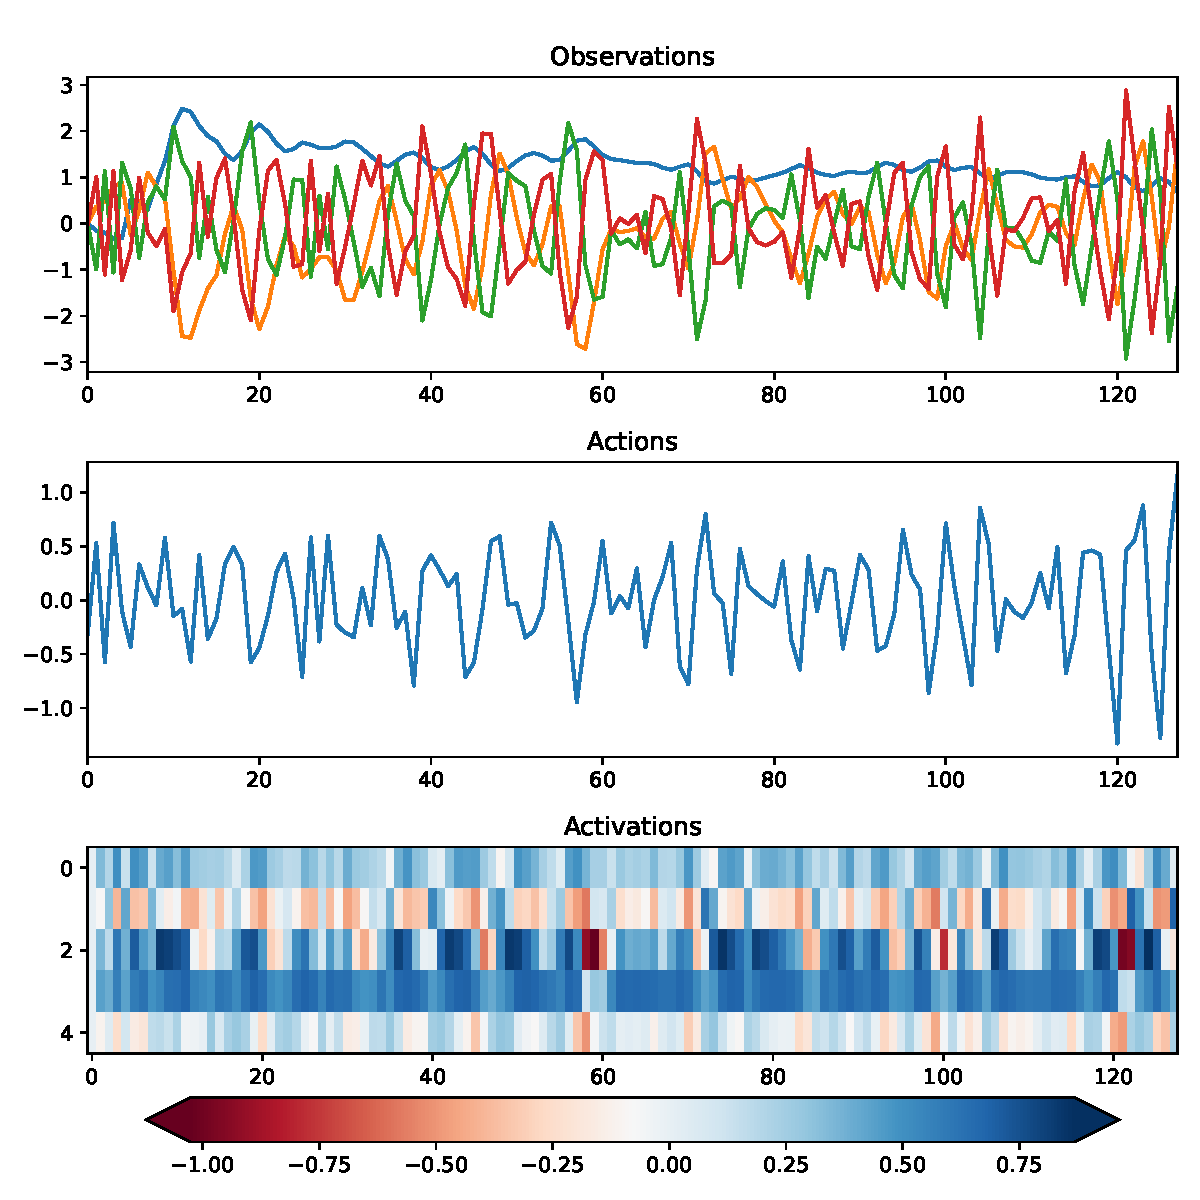
\includegraphics[width=0.4\textwidth]{figures/5n_solution.pdf}
    \caption{Visualization of (from the top down) observation, action and neuron activations together for a $5$ neuron LTC cell trained with PPO on a cart-pole \textit{Mujoco} environment. The activation plot is structured as follows, each row correspond to a single neuron is colored along the $t$ horizontal axis according to the activation $x_i$ of that neuron at time $t$.}
    \label{fig:5n_episode}
\end{figure}

We find that the LTC cell trained with PPO can find efficient solutions to the cart-pole problem, but that it does so with a particularly low sample efficiency (compared to a reference \textit{Multi-Layer Perceptron} ({MLP}) model trained with a perceptron). On the other hand the amount of neurons required to achieve a good solution is extremely low compared to the amount of MLP neurons that would be required for solving the problem with a {MLP} model. This ability of the model to find low-neuron count solutions isn't of interest for computational reasons (recall the the number of parameters per neuron is much higher than in the case of an MLP) but may prove interesting as that low neuron count may make the system easier to interpret. 

\subsection{The 5 neuron solution, trying to make sense of the activations}
\label{sec:5-neurons}

\begin{figure}[h!]
    \centering
    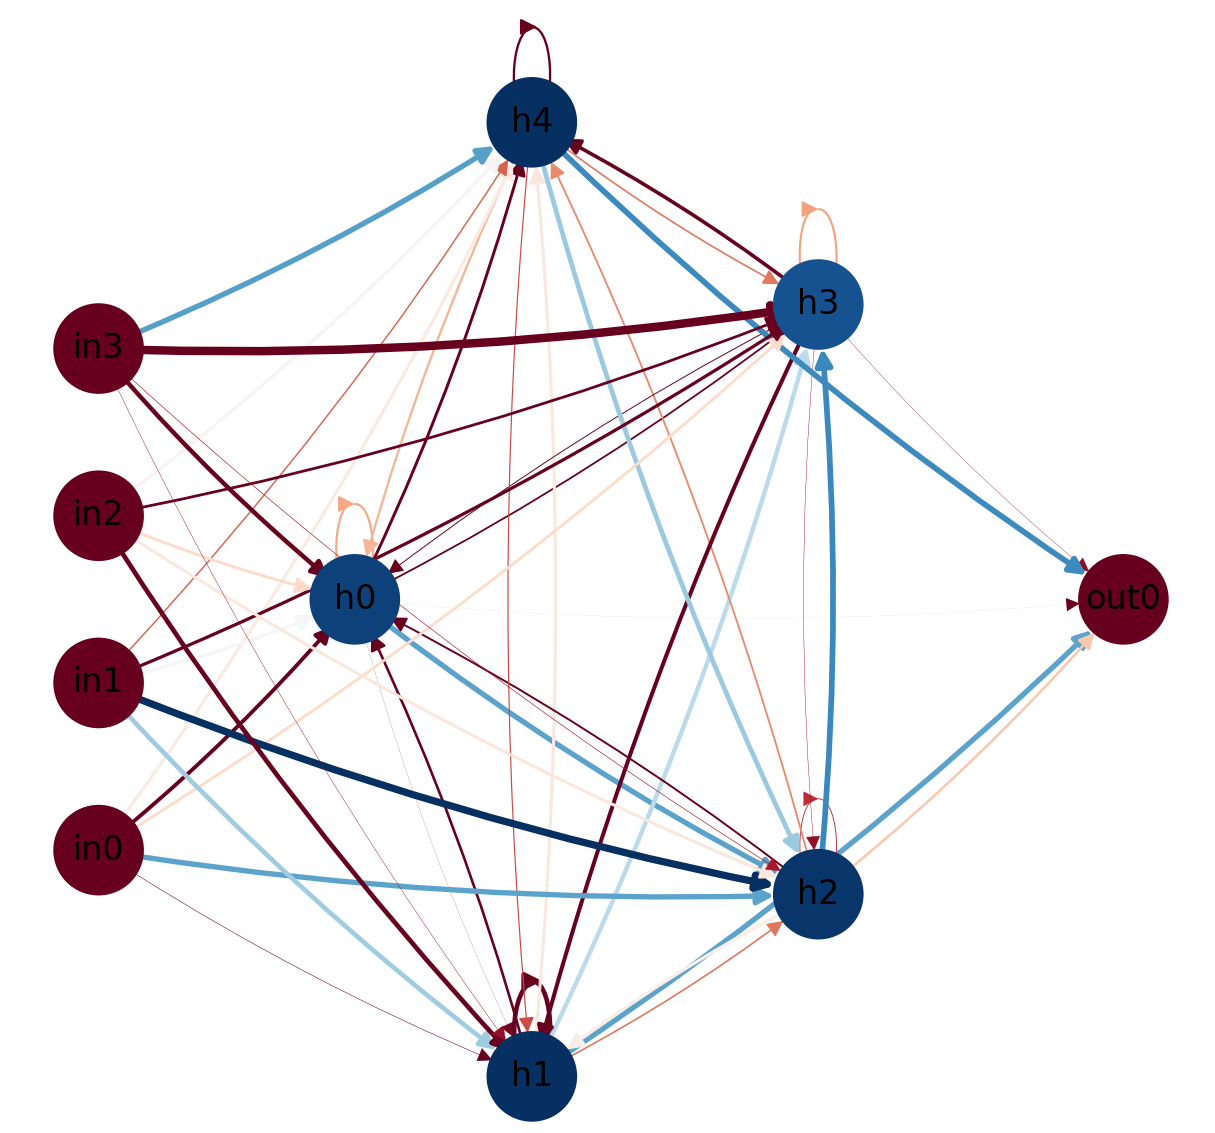
\includegraphics[width=0.4\textwidth]{figures/5n_schematic.png}
    \caption{Representation of the $5$ neuron LTC cell. Connections are colored and scaled with respect to their intensities, the inner-neurons are colored with respect to their time-constants.}
    \label{fig:5n_schematic}
\end{figure}

The lowest number of neuron that actually could solve the cart-pole problem is $5$. The solution obtained with $5$ neurons actually leads to a relatively unstable control (the cart-pole oscillates a lot under that policy, as can be observed in figure \ref{fig:5n_episode}) but it is interesting because the policy can be investigated relatively easily, which we try to do in this section.  We plot out connections of the trained cell in figure \ref{fig:5n_schematic}.\\

\begin{figure}[h!]
    \centering
    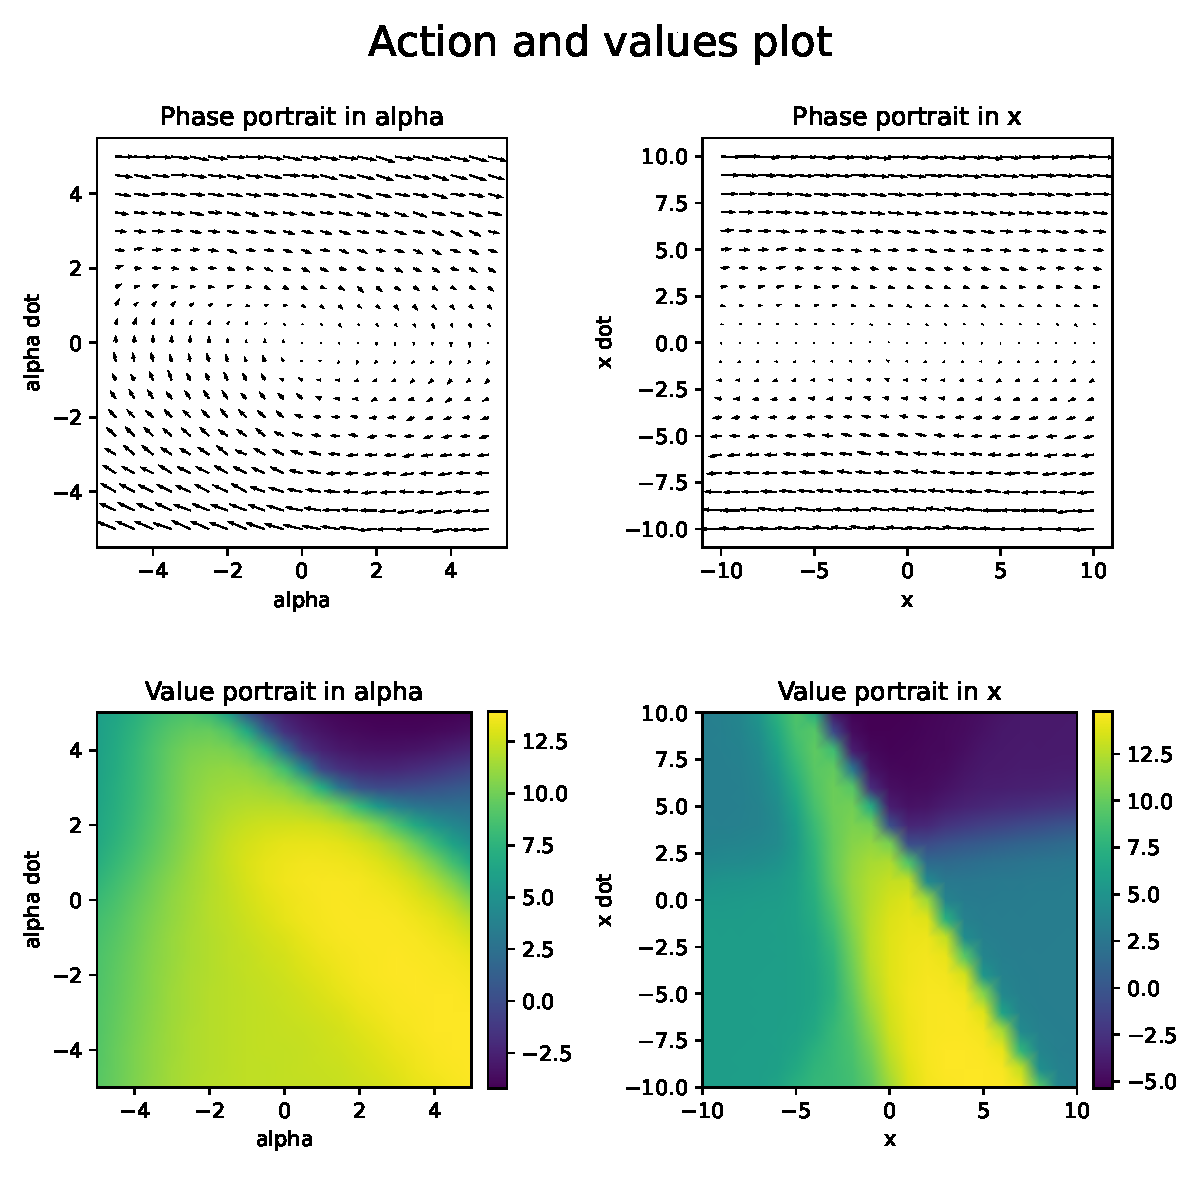
\includegraphics[width=0.4\textwidth]{figures/5n_portrait.pdf}
    \caption{Characterization of a 5-neuron LTC-cell policy. Phase portraits (top) and value portraits (down) in the pole angle phase space $\alpha,\dot{\alpha}$ (left) and cart position phase space (right).}
    \label{fig:5n_portrait}
\end{figure}

The cart-pole trained policies take a $4$-dimensional vector as an input, so plotting a visual representation of their behavior is non trivial. One approach that we can to generate two two-dimensional plots where we compute responses of the policy and value nets to observations in either $\alpha,\dot{\alpha}$-space or $x,\dot{x}$-space. 
In both case we fix both the other two observation variables (respectively $x,\dot{x}$ or $\alpha,\dot{\alpha}$) to $0$. For now we also choose to fix the inner states of all the neurons to $0$ (we disregard self-connections). 
This enables us to plot out a \textit{portrait} of how our LTC cell responds to various observations from it's environment (we call these plots \textit{portraits} as we are trying to interpret these plots in a similar fashion to how phase-portraits are used in the dynamical system theory literature). We plot out both the output of the policy network and of the value network. We use the policy network output to plot a phase-portrait as a vector field where for each point $(\alpha,\dot{\alpha})$ we plot a vector $(\alpha,u)$ and for each point $(x,\dot{x})$ we plot a vector $(x,u)$ and the output of the value network (we construct this plot in hope of identifying sinks and sources in the flow of the closed loop dynamical system). In the case of the value network we simply plot out the estimated value for each point in the space we investigate, this gives us an idea of "\textit{how good does the policy thinks being in a given state is}", we call these plots "\textit{value portraits}". \\



The \textit{portraits} we computed for the $5$-neuron LTC cell (figure \ref{fig:5n_portrait}), allow us to identify a sink at the point $(0,0)$ in the pole-angle phase space (see the top left plot in figure \ref{fig:5n_portrait}), which tends to indicate that our policy is tends to stabilize the cart-pole system around that point (which is what is to be expected). On the other hand the phase portrait in the cart-position phase-space doesn't show any clearly defined sink, this confirms what we observe when running simulations: the policy doesn't center the cart-pole's movements around the origin. This is suboptimal and shows that the $5$-neuron policy isn't fully converged. \\

\begin{figure}[h!]
    \centering
    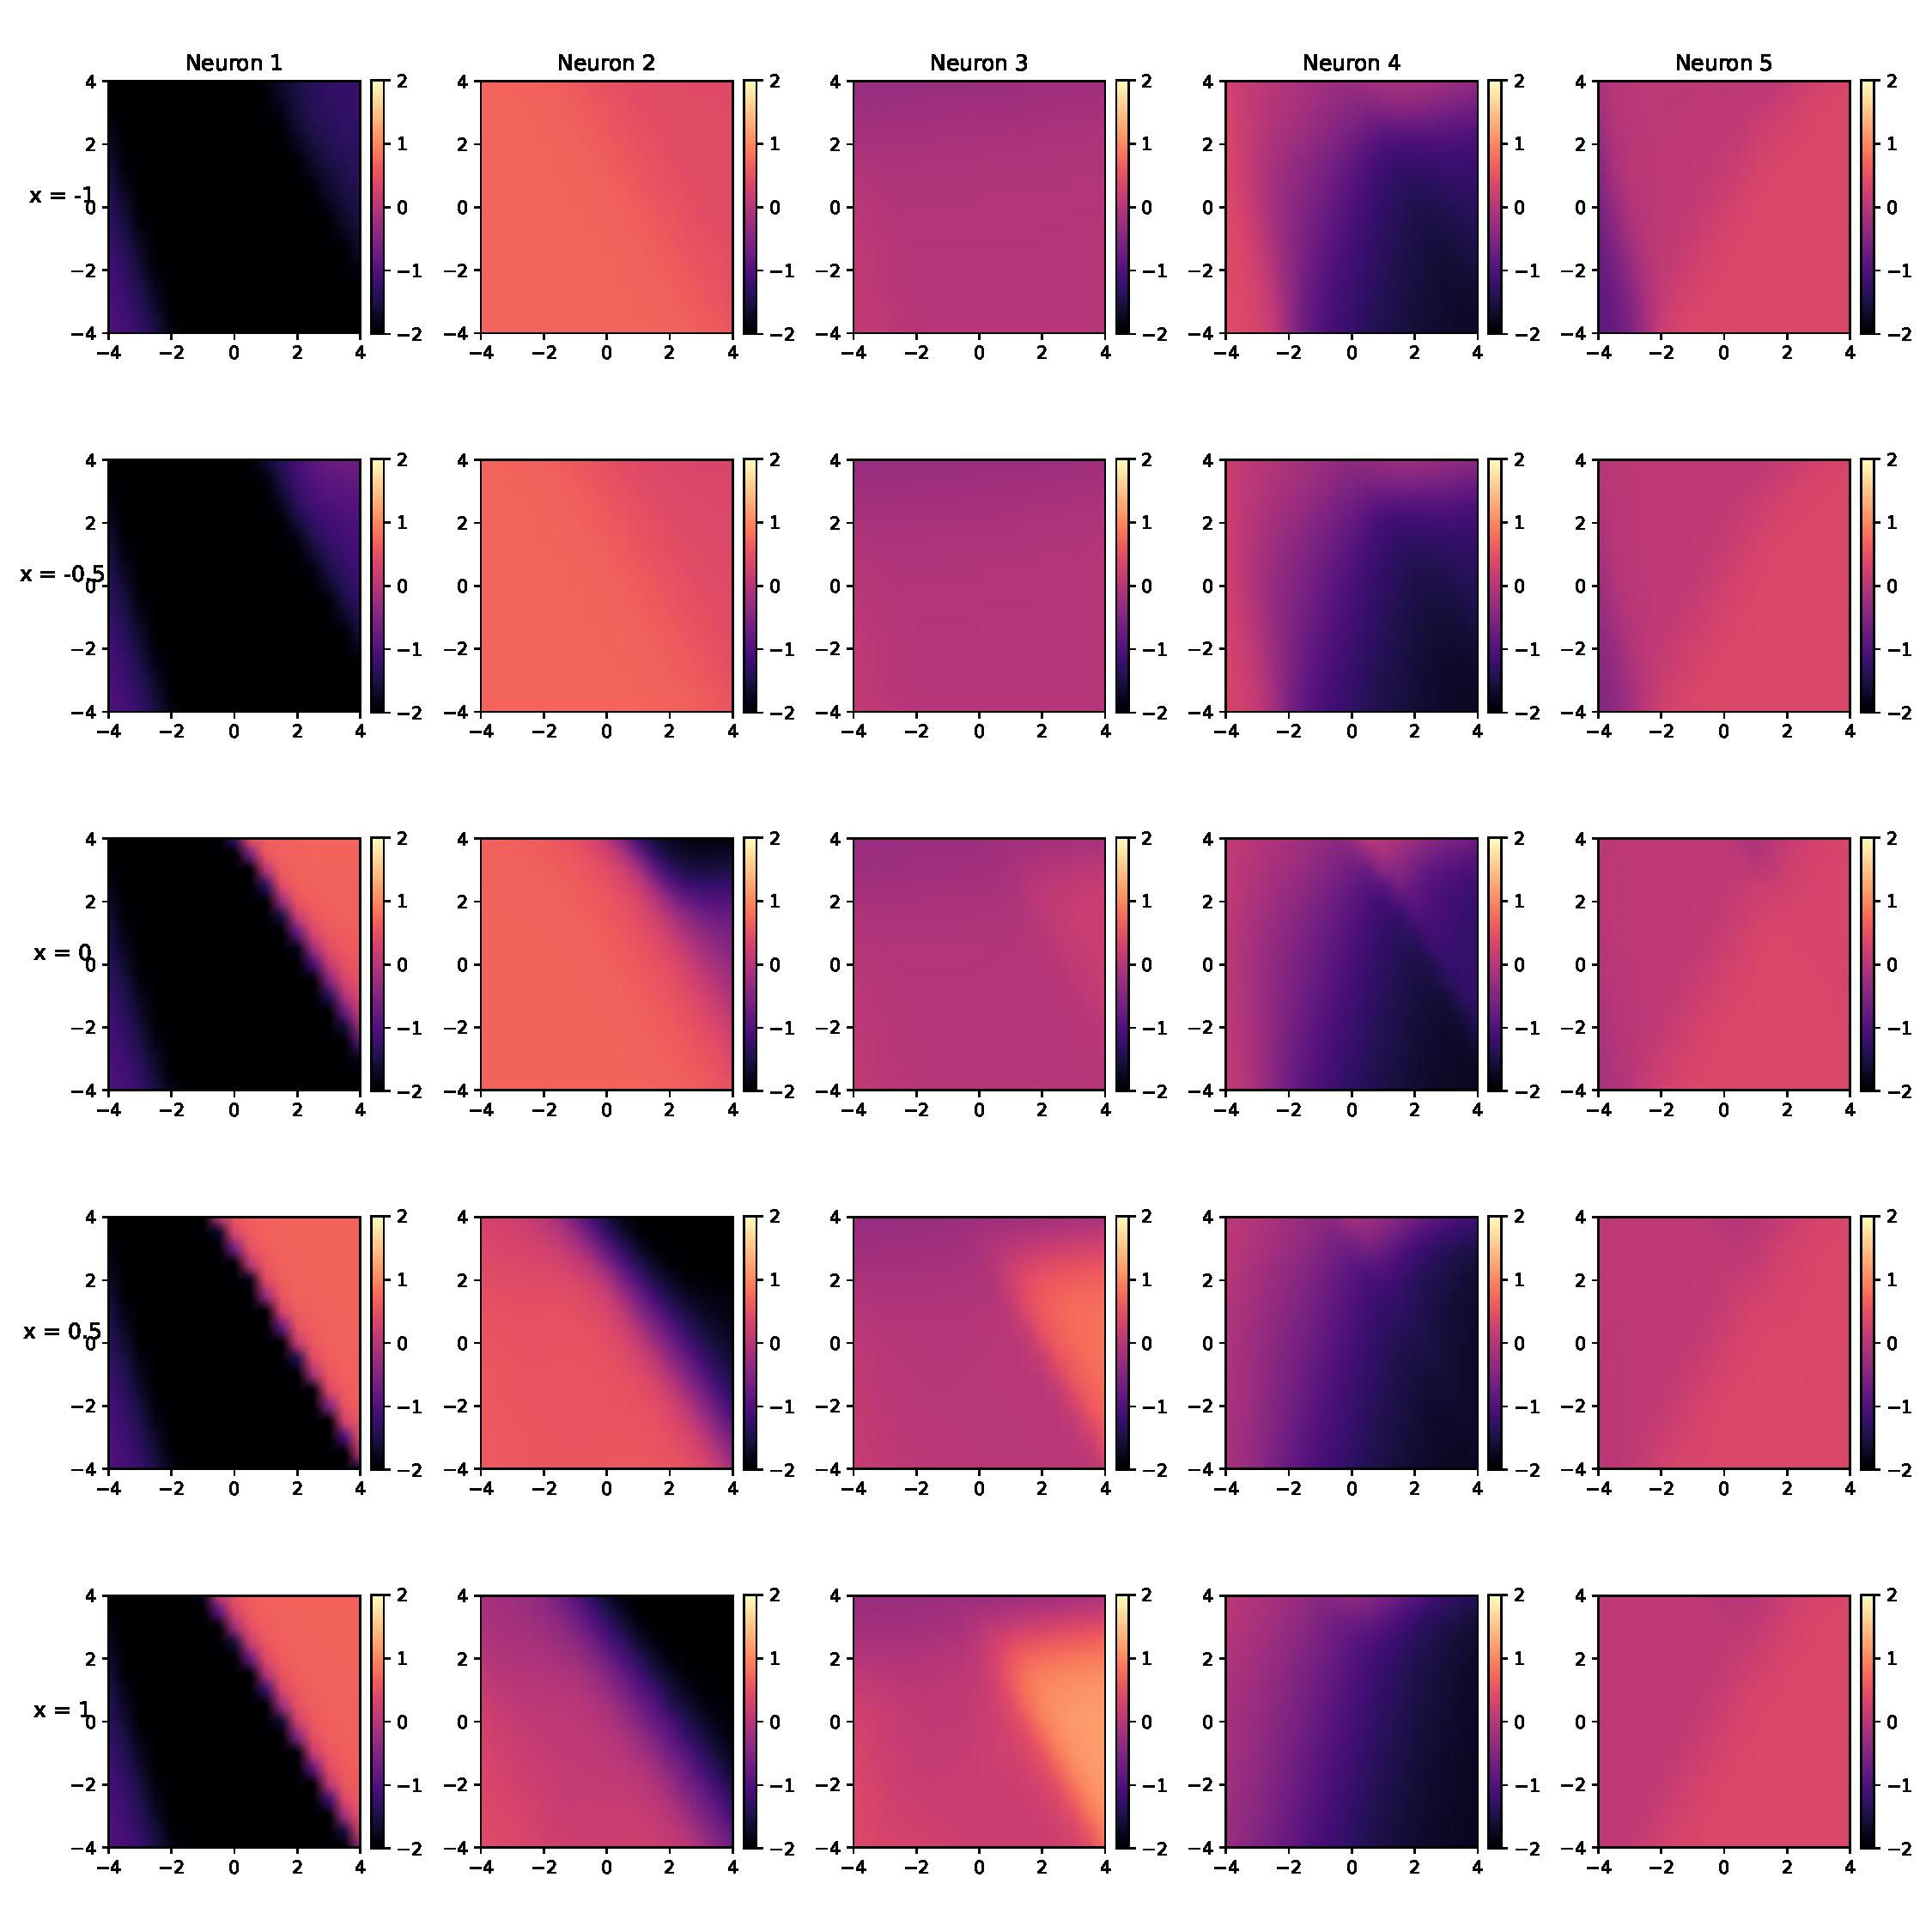
\includegraphics[width=0.4\textwidth]{figures/5n_pnr.pdf}
    \caption{Pole angle phase-space response of each of the $5$ neurons of the cells with various inner-states activations $x_i$. From left-to-right: responses of neurons $1$-to-$5$. From top-to-bottom: responses of the neurons with inner states $-1$-to-$1$.}
    \label{fig:5n_invidual_responses}
\end{figure}

Furthermore, the value portraits from figure \ref{fig:5n_portrait} show asymmetric value estimations which further indicates that the policy shows hasn't completely converged (the control problem is symmetric so one should expect a converged value net to predict a symmetric performance). \\

This approach isn't sufficient to characterize the response of the $5$-neuron cell as it completely disregards the influence of the inner-neuron states, it also fails to interpret the behavior of different neurons. In order to build a deeper understanding of the cell we investigate the response of individual neurons to different inputs and to various activations. We decide to focus on the policy network and on the pole-angle phase space, we construct a plot for each of the $5$-neuron and for various inner-states activations. The resulting plot is presented in figure \ref{fig:5n_invidual_responses}. \\

The resulting plot shows a clear influence of the inner states of the neurons influence (although the influence of the angle seems to dominate for every neuron, this is also a tendency which we observe when comparing the influence of angle compared to position). This indicates that the neuron make some use of the recurrent connections. 


\subsection{Neuron Count Experiments}
We run experiments with various neuron counts ($5,6,7,8,16,$ and $32$ neurons). The main questions we aim to answer with such a protocol are "\textit{Is there a minimum neuron count to solve such a problem?}" (and how different is it from the minimum neuron count with a perceptron) and "\textit{how does the neuron count affect the quality of solution?}". \\

The first question, the minimum neuron count required to solve cart-pole seems to be somewhere around $5$ (the cell that we investigated in section \ref{sec:5-neurons} is the lowest count for which we could observe convergence).


\subsection{Sample efficiency}
\textbf{TODO : Influence of nc and mask?}
\begin{figure}[h!]
    \centering
    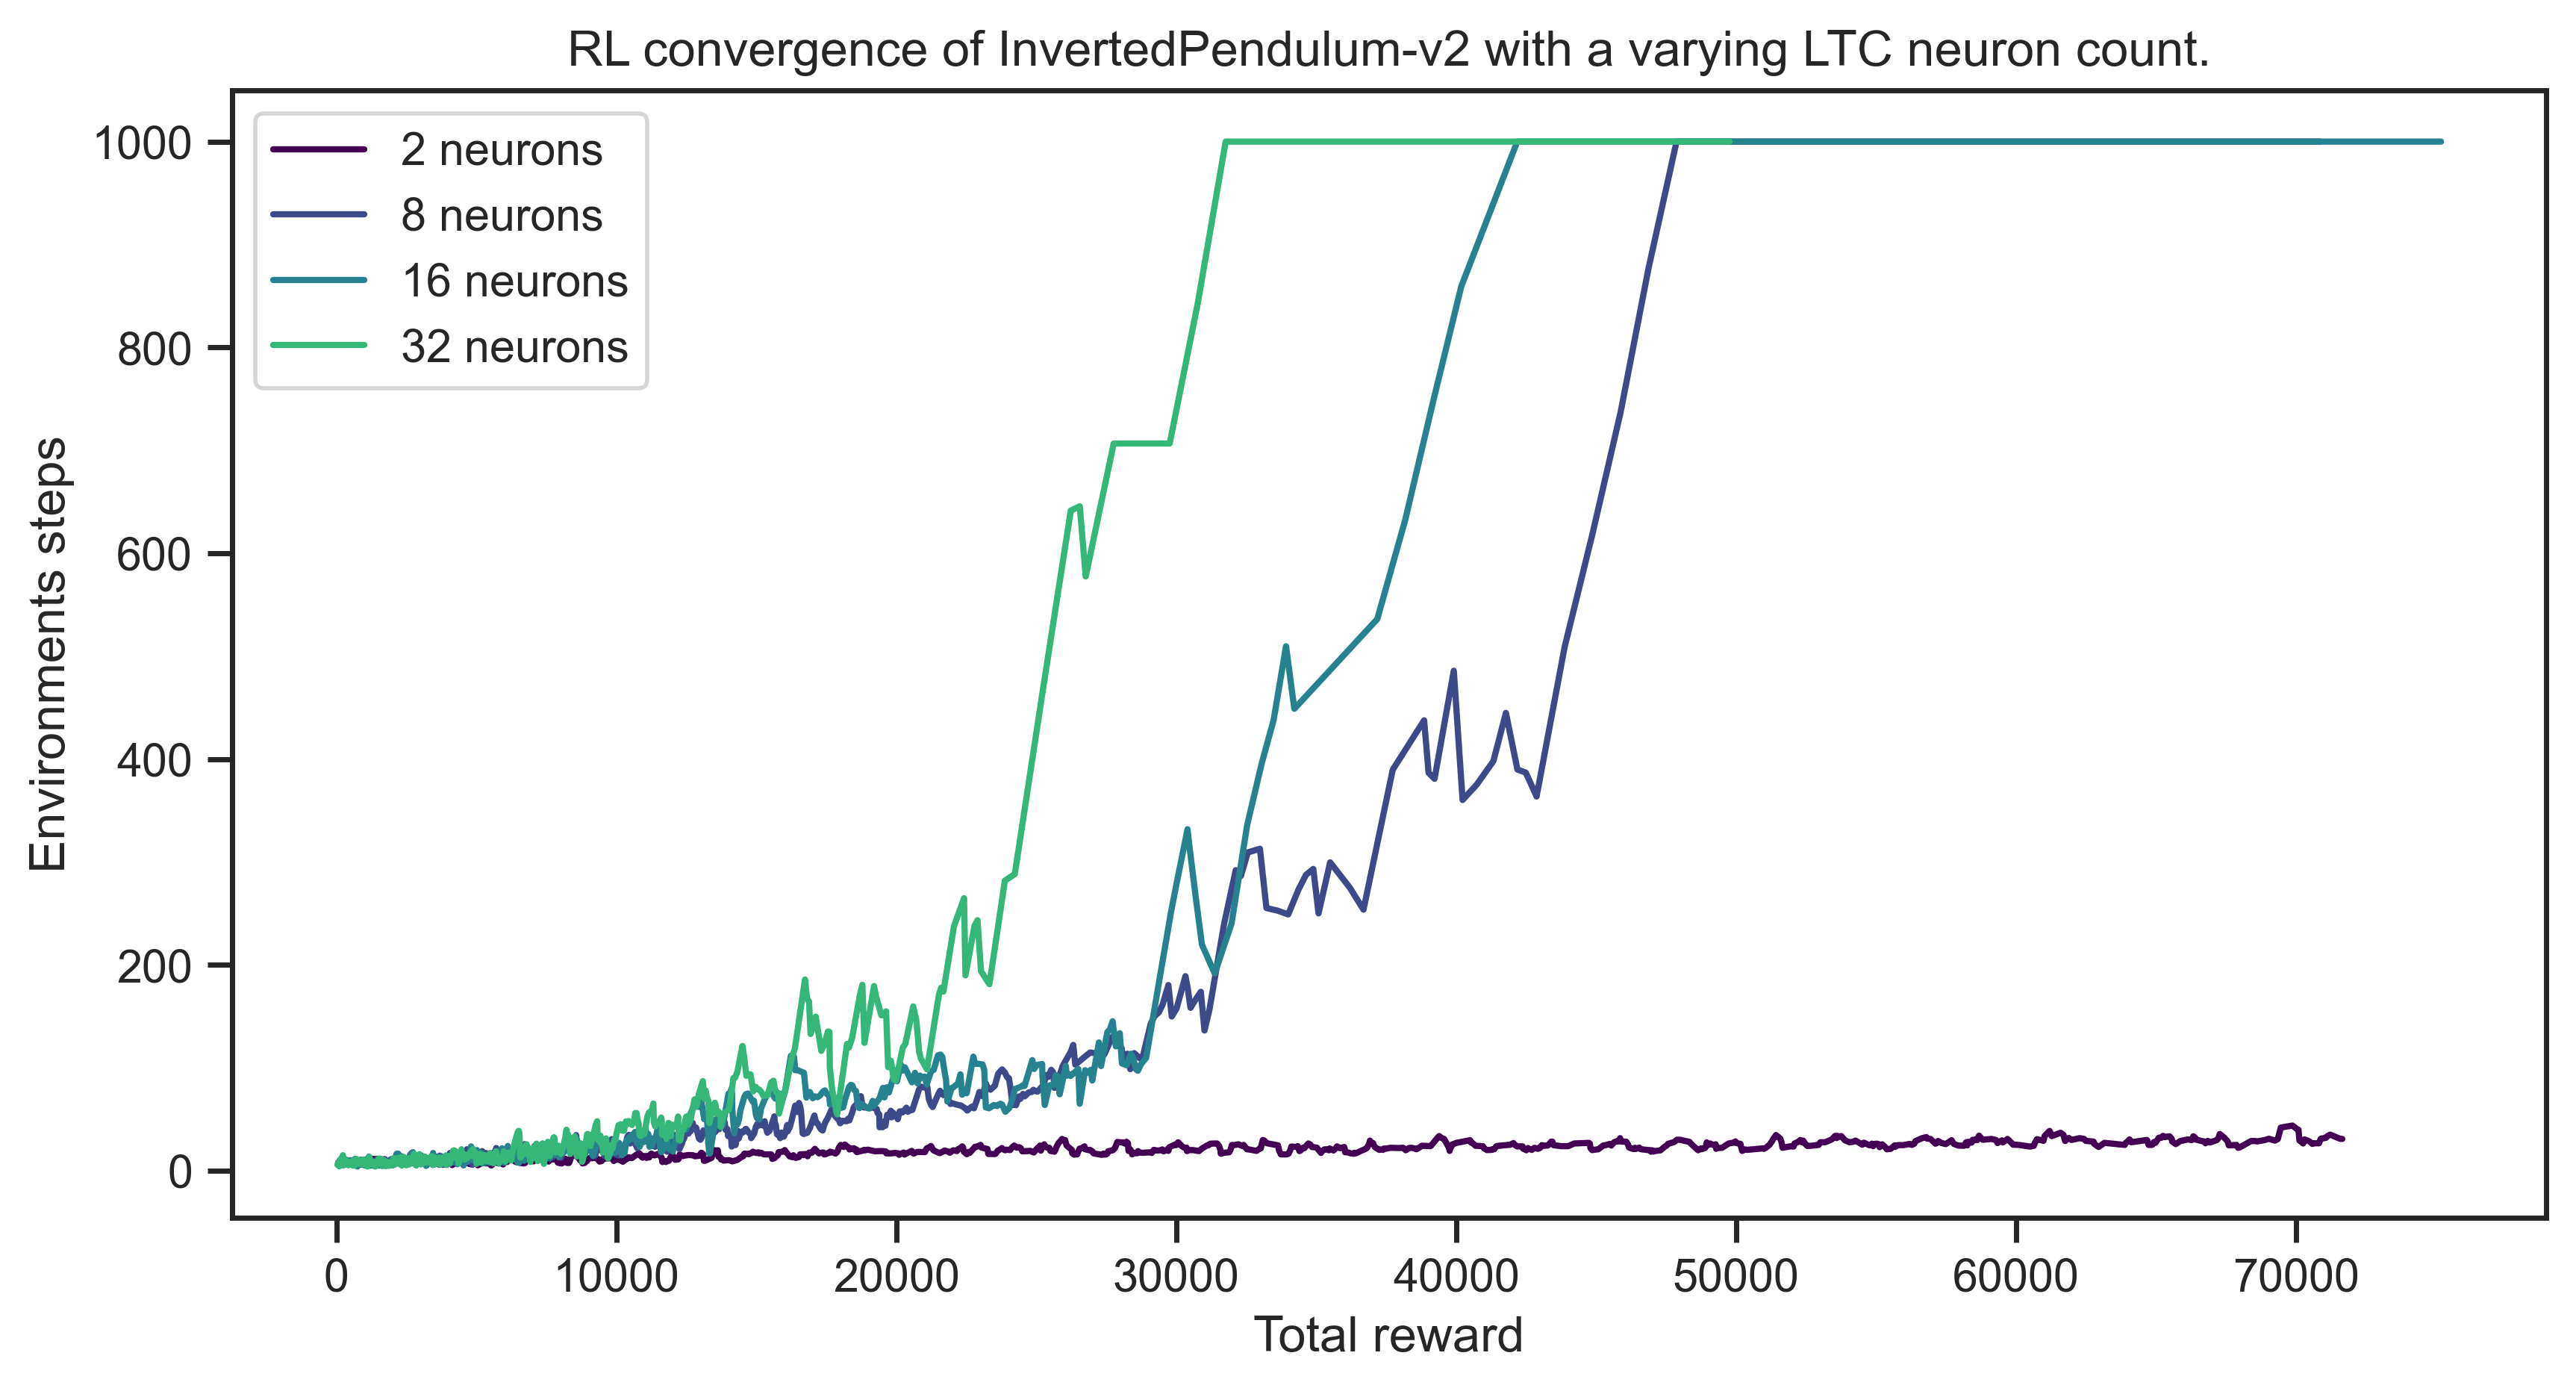
\includegraphics[width=0.45\textwidth]{figures/convergence_rate.png}
    \caption{}
\end{figure}

\subsection{Resilience to noise?}
\textbf{TODO : Influence of nc and mask?}

\subsection{Discussion of the results}
\textbf{TODO : Discuss the usability of the learned policies, what can we infer from this}


\subsection{Further work section}
\textbf{TODO : Discuss what I didn't have time to do?}